
\begin{comment}
\begin{frame}{CZ-PL}
\begin{figure}
\justifying
\begin{itemize}
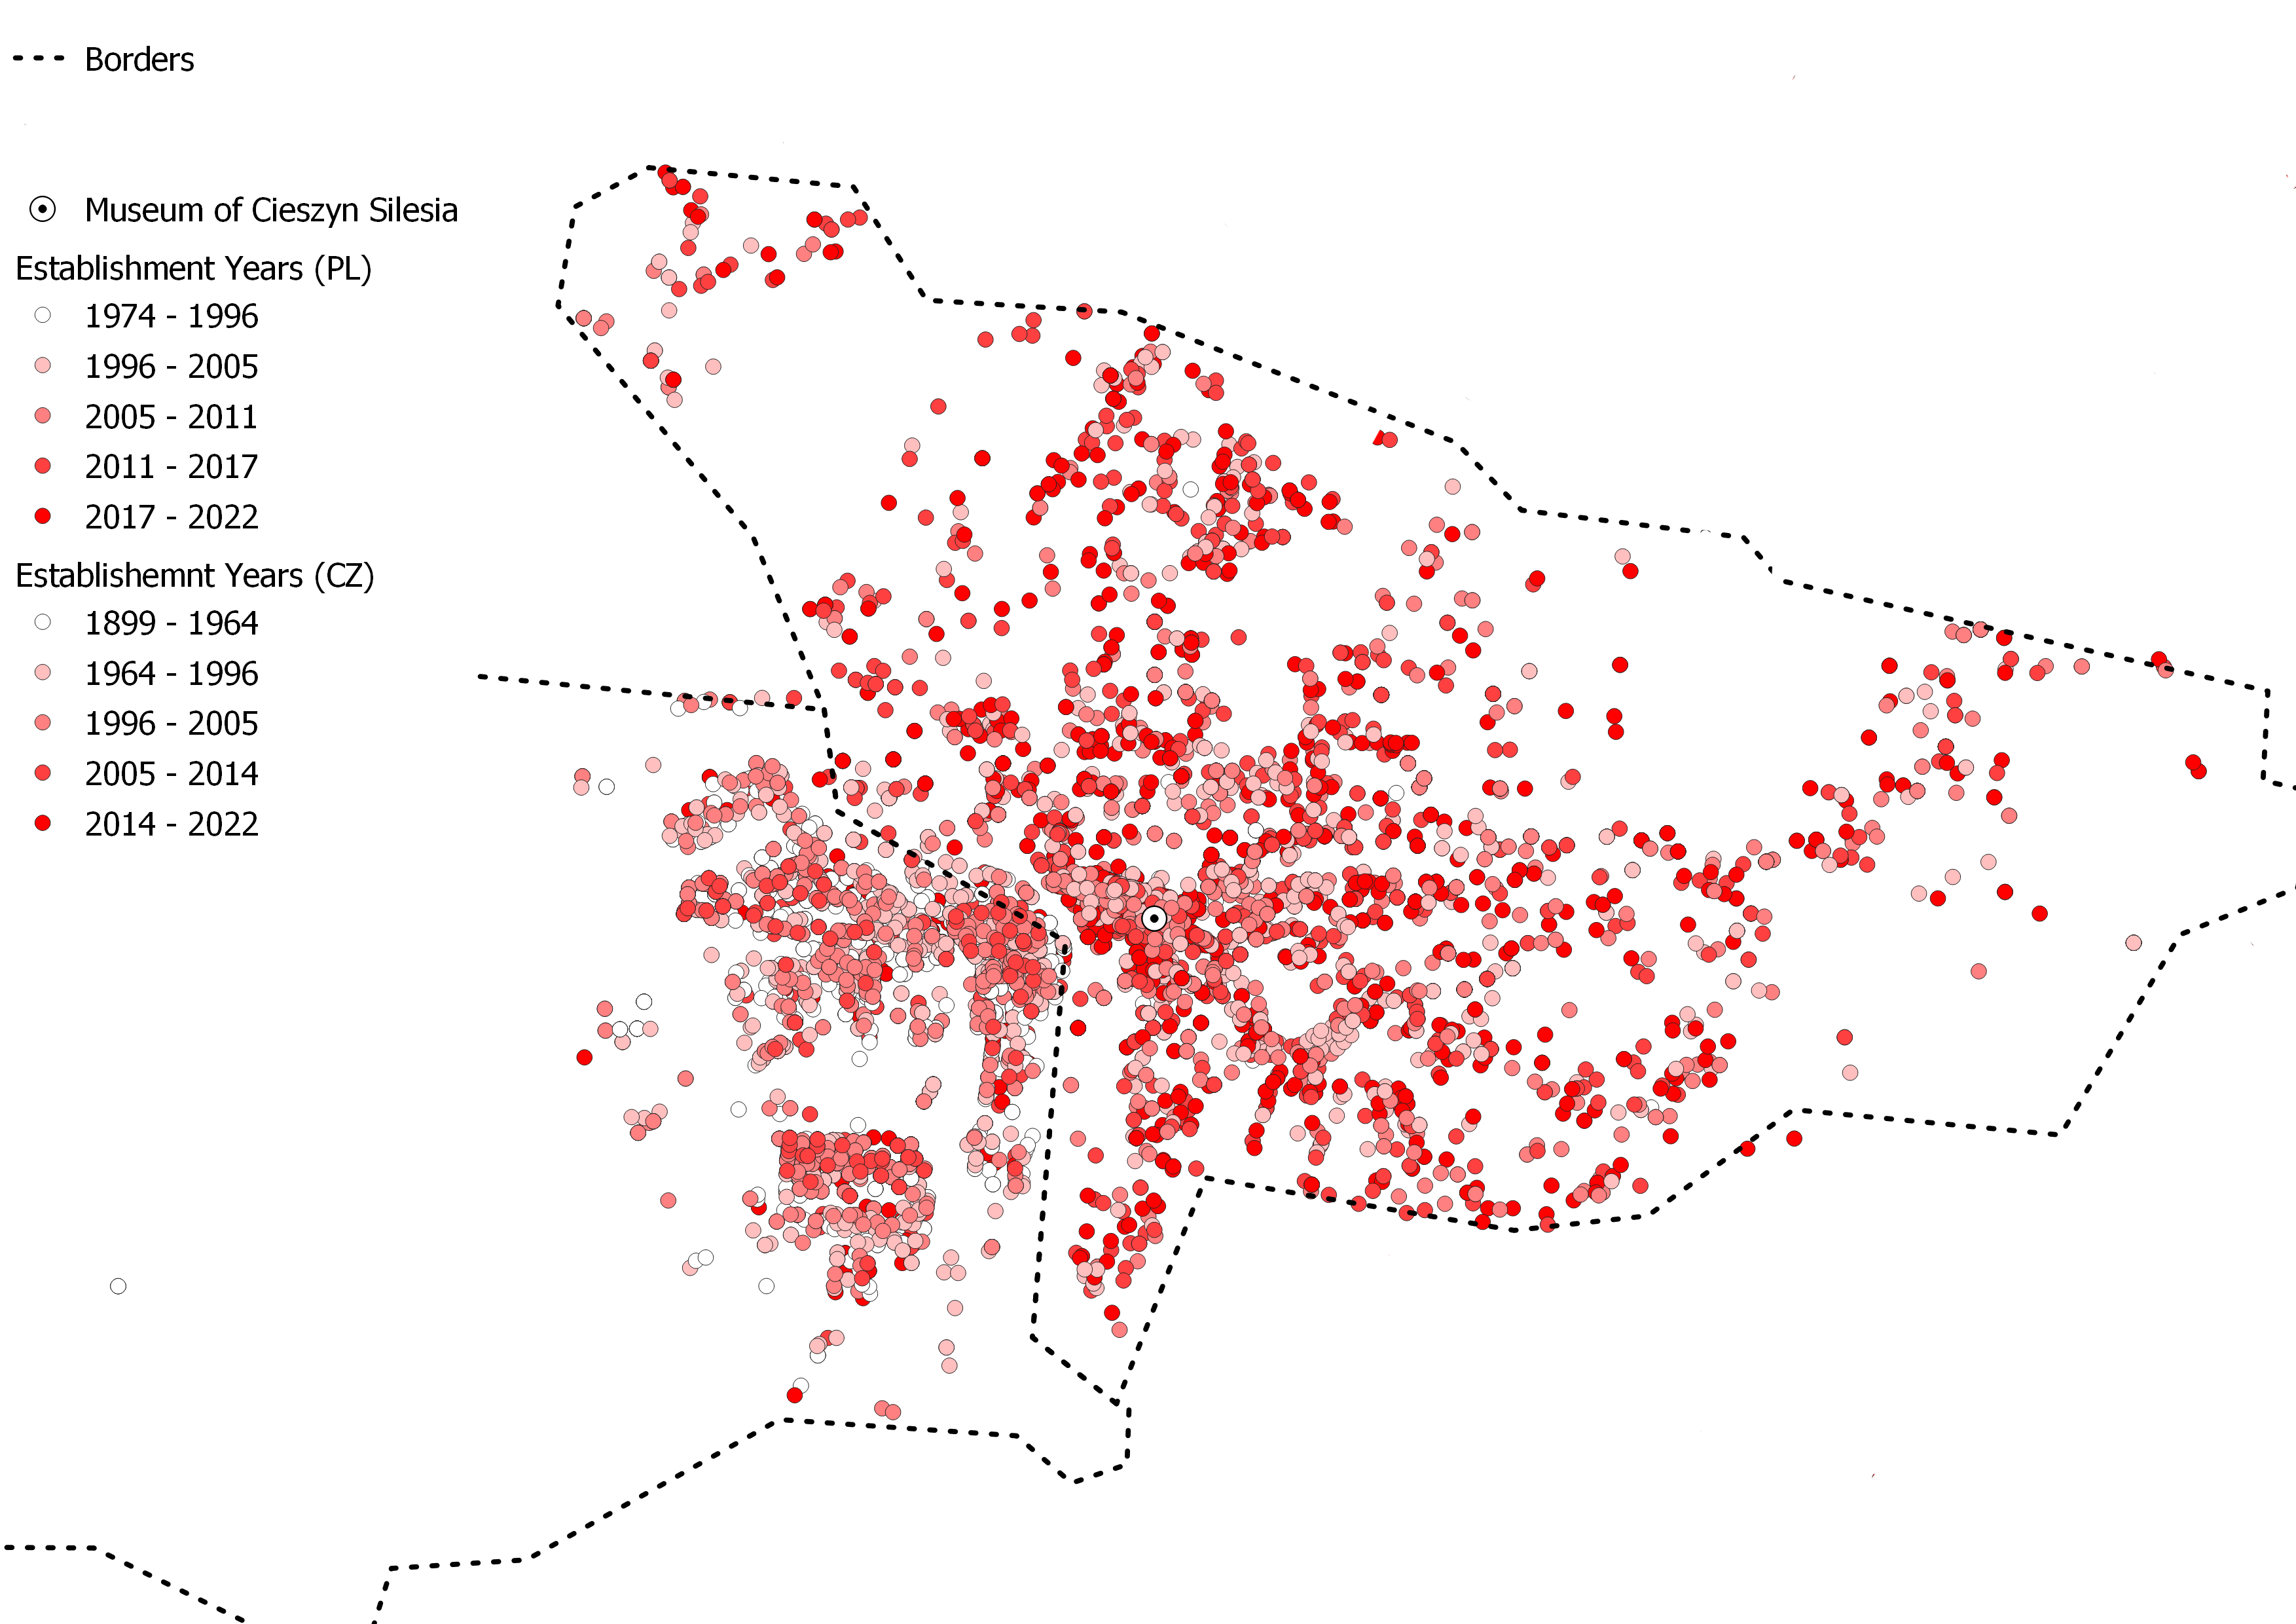
\includegraphics[scale=0.35]{cz_pl.png}
\end{itemize}
\end{figure}
\end{frame}





\begin{frame}{CZ}
\begin{figure}
\justifying
\begin{itemize}
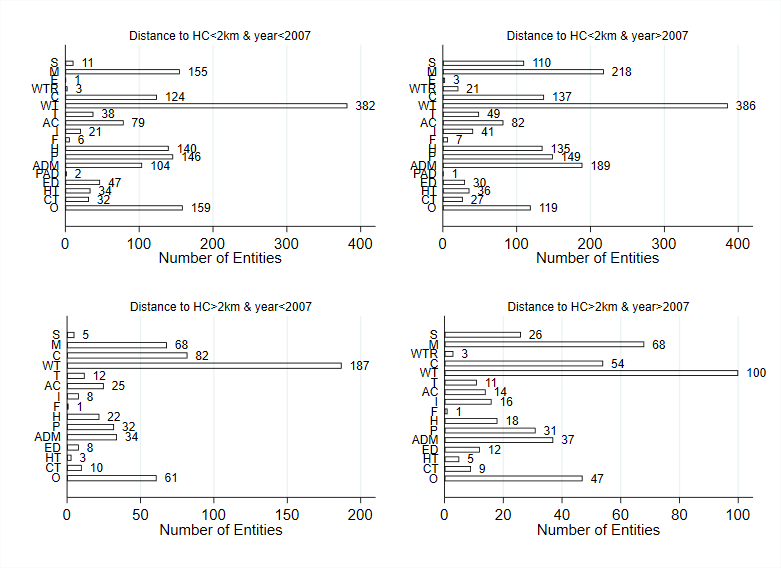
\includegraphics[scale=0.35]{cz.png}
\end{itemize}
\end{figure}
\end{frame}

\begin{frame}{PL}
\begin{figure}
\justifying
\begin{itemize}
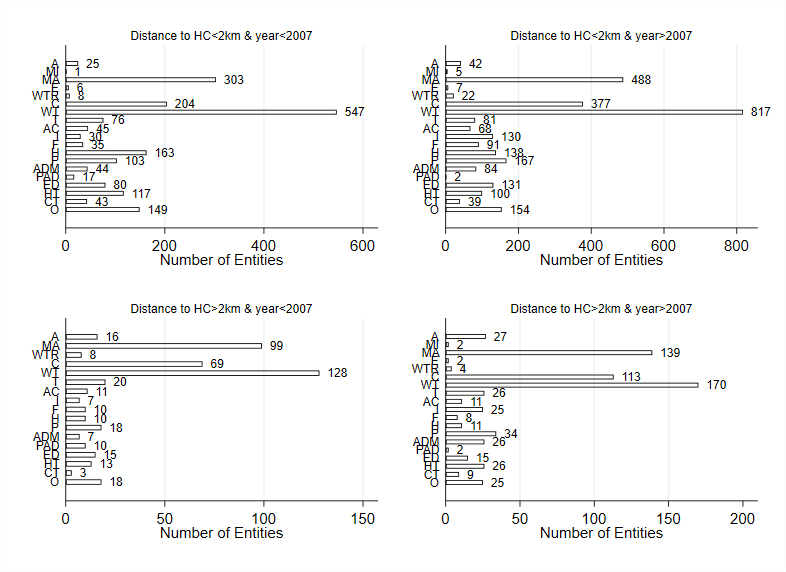
\includegraphics[scale=0.35]{pl.png}
\end{itemize}
\end{figure}
\end{frame}

\begin{frame}{Empirical Model I}
\textbf{Hypothesis I:} Economic activities become denser near pre-division historical centers than in other zones after 2008
\begin{equation*}
\justifying log(NTL+0.01)_{it}=\alpha+\beta Sch_{t} +\gamma Sch_{t} * HCC_{i}+D_{i}+D_{t}+D_{s}+\epsilon_{it}
\end{equation*}
\justifying
\begin{itemize}

\item $log(NTL+0.01)_{it}$ represents the percentage changes in stable nightlights -  a proxy of changes in local economic outcome in grid cell $i$ at time $t$
\item $HCC_{i}$ is the proximity from grid cell $i$ to pre-division historical city center, measured in \textit{km}
\item \small $\gamma$ explains how NTL changes in areas close to the historical centers after removing all border barriers
\item $D_{t}$, $D_{i}$ and $D_{s}$ are year,  pixel, and satellite fixed effects
\end{itemize}
\end{frame}




\begin{frame}{Results I}
\begin{table}[H]
\centering
\small
\def\sym#1{\ifmmode^{#1}\else\(^{#1}\)\fi}
\caption{The Effect of Removing Borders on NTL in Divided Cities \label{reg1}}
\begin{tabular}{l*{3}{D{.}{.}{-1}}}
\toprule
  Dep: \textit{Stable Nightlights}
  &\multicolumn{1}{c}{ ln(NTL)}               &\multicolumn{1}{c}{NTL}         \\
\midrule
\midrule
Schengen $\times$ Proximity to HCC&    0.004\sym{***}&         0.378\sym{***}\\
                          &     (0.001)         &     (0.011)         \\
                    \hline
                    \hline
Schengen     &       0.099\sym{***}&          3.616\sym{***}\\
                    &     (0.023)                &     (0.173)         \\
\addlinespace
Constant            &      -0.207\sym{***}&         13.910\sym{***}\\
                    &     (0.020)                 &     (0.091)         \\
\midrule
Year FE              &        \checkmark        &        \checkmark \\
Satellite FE             &       \checkmark       &        \checkmark \\
Pixel FE               &       \checkmark         &        \checkmark \\ 
\midrule
Observations        &       74,729                 &       74,729         \\
\end{tabular}
\end{table}
    
\end{frame}

\begin{comment}
\begin{frame}{Empirical Model II \& III}
\begin{itemize}
\justifying
\item \textbf{Hypothesis II}: Newly established economic entities are highly concentrated near pre-division historical centers after free movement of people was allowed in 2008 
\begin{itemize}
    \item concentration does not appear near pre-division centers due to 2004 Eastern Enlargement, i.e. after solely boarder market access
\end{itemize}
\end{itemize}
\vspace{0.5cm}
\begin{equation}
\begin{split}
    D(Entry Year_{i} \geq 2008)=\alpha+ \beta ProximityToHCC_{i}+D_i+\epsilon_{i}
    \end{split}
\end{equation}
vs.
\begin{equation}
\begin{split}
    D(Entry Year_{i} \geq 2004)=\alpha+ \beta ProximityToHCC_{i}+D_i+\epsilon_{i}
    \end{split}
\end{equation}
\end{frame}

\begin{frame}{Results II}
\begin{table}[]
\caption{Concentration of Economic Entities Established in 1900-2022 \label{reg1}}
\small
\begin{tabular}{|l|llll|}
\hline
       Dep: \textit{Entry Year}      &  D( \leq 1990)          
                 &   D(\geq 2004)                                           
                 &  D( \geq 2008)                                                                            
                 &   D( \geq 2011)                          \\
\hline
\hline
Proximity to HCC &
\begin{tabular}[c]{@{}l@{}}-0.006**\\ (0.003)\end{tabular} &
\begin{tabular}[c]{@{}l@{}}-0.002\\ (0.002)\end{tabular} & 
\begin{tabular}[c]{@{}l@{}}0.007***\\ (0.002)\end{tabular} & \begin{tabular}[c]{@{}l@{}}0.025***\\ (0.002)\end{tabular} \\
\hline
\hline
Con.             & \checkmark                                                          & \checkmark                                                           & \checkmark                                                        & \checkmark                                                           \\
City FE          & \checkmark                                                           & \checkmark                                                           & \checkmark                                                         & \checkmark                                                          \\
\hline
N                &   10,611                                                    & 39,625                                                     & 39,625                                                   & 39,625   \\                                              
\hline
\end{tabular}
\end{table}

\begin{itemize}
\item \footnotesize $D(.)$ dummies are constructed based on establishment years of economic entities 
\item \footnotesize Probit model estimation
\end{itemize}
\end{frame}



\begin{frame}{Channels}
I account for two main channels through which the market concentration appear after all types of border barriers were removed between divided European border cities in 2008
\vspace{0.6cm}
\begin{itemize}
    \item \textbf{Sectors}: type of registered economic entity
    \vspace{0.3cm}
    \item \textbf{Culture}: language \& cultural similarities
\end{itemize}
\end{frame}

    
\begin{frame}{Channel I: Sectors}
Firms in \textbf{consumption} sector that aim to provide services to customers and are not engaged in \textbf{production} are more exposed to removing of borders because free movement policy allows foreigners and locals  to mobile freely across borders. 

\begin{equation*}
    D(Entry Year_{i} \geq 2008)=\alpha+ \beta ProximityToHCC_{i}\times Sectors_{i} +D_i+\epsilon_{i}
\end{equation*}

\begin{itemize}
\justifying
    \item $D(Entry Year_{i} \geq 2008)$ is a dummy variable taking a value of one if economic entity was established after 2007
    \item $ProximityToHCC_{i}$ represents distance to pre-division center 
    \item $Sectors_{i}$ represents  classification of newly established  economic entities
\end{itemize}
\end{frame}



\begin{frame}{Channel I: Sectoral Decomposition}
\footnotesize
\begin{table}[]
\caption{Regression Coefficients by Sectors}
\begin{tabular}{l|l|l||l|l|l}
\hline
\hline
     Dep: $D(\geq 2008)$        & Coeff.     & N    &         Dep: $D(\geq 2008)$         & Coeff.     & N    \\
              \hline
\textbf{Agriculture}   & 0.082***  & 531  & Information    & 0.006     & 1132 \\
Mining        & 0.152   & 25   & Finance        & -0.015    & 584  \\
Manufacturing & 0.010   & 4197 & Real Estate    & 0.010     & 2142 \\
Electricity   & -0.193*** & 131  & Professional   & -0.027*** & 4124 \\
\textbf{Water}         & 0.081**   & 153  & Administrative & -0.068*** & 1597 \\
Construction  & -0.009    & 3990 & Public         & 0.128     & 73   \\
\textbf{Trade}         & 0.03***   & 9200 & Education      & 0.003     & 891  \\
Transport     & -0.117*** & 1956 & \textbf{Health}         & 0.003***  & 1011 \\
\textbf{Accommodation} & 0.069***  & 1235 & Culture        & -0.005    & 1096 \\
 \hline  
 \hline
\end{tabular}
\end{table}
\end{frame}

    \begin{frame}{Channel II: Culture \& Language}

Interreg A cross-border cooperation survey:

\begin{itemize}
\justifying
    \item \textit{Thinking about the cooperation between [Country A] and [Cross-
Border Country B], to what extent are language differences \& cultural differences a major problem?}

\end{itemize}

\begin{equation*}
    D(Entry Year_{i} \geq 2008)=\alpha+ \beta ProximityToHCC_{i}\times Similarity_{i} +D_i+\epsilon_{i}
\end{equation*}
\begin{itemize}
\justifying
    \item $Similarity_{i}$ - is a dummy and takes one if the calculated share of respondents in NUTS3 region where divided city is located is above average; where respondents think that language and cultural differences are not major problems in cross-border cooperation
\end{itemize}
    
\end{frame}


    
\begin{frame}{Channel II: Culture \& Language}
\small
\begin{table}
\caption{Language and Cultural Similarity in Divided Cities}
\begin{tabular}{l*{1}{c}}
\hline\hline
Dep: D(Entry Year \geq 2008)  &\multicolumn{1}{c}{(1)}\\
  &\multicolumn{1}{c}{}\\
\hline
Language \& Cultural Similarity X HCC &      0.0109\sym{**}  \\
            &      (2.49)         \\
            \hline

Proximity to HCC       &    -0.00213         \\
            &     (-0.56)         \\
 {Language \& Cultural Similarity}    &      0.0199         \\
            &      (0.58)         \\

Con.     &       0.209\sym{***}\\
            &      (7.95)         \\
\hline
\(N\)       &       39,625         \\
\hline\hline
\end{tabular}
\end{table}
\end{frame}
\end{comment}